\section{Análisis de señales}

\subsection{Señal Cuadrada}

Para esta sección se utilizó una señal cuadrada de $350mV$ y con un $DC$ del 50\%. Esta señal fue generada con el generador de señales Agilent.

\subsubsection{Cálculo Analítico}

Sea una señal cuadrada $f(t)$ de amplitud $A$ y frecuencia $f_0$, el desarrollo en serie de Fourier para esta señal es:

\begin{equation}
    f(t)=\frac{A}{2}+\sum_{n=1}^{\infty} \frac{2A}{n\pi}sin(2\pi n f_0t)
    \label{eq:fouriercuadrada}
\end{equation}

Luego, $X_n=\frac{2A}{n\pi}$ representan los coeficientes de la serie de Fourier de la onda cuadrada para $n>1$ Notemos, además, que para múltiplos pares de la frecuencia fundamental la señal se anula. Luego se verán únicamente armónicos impares en el espectro.

\subsubsection{Simulación del Espectro}

Se realizó una simulación del espectro de una señal cuadrada con frecuencia $1 MHz$ y amplitud $350 mV_{pp}$. En la figura (\ref{fig:simcuad}) se puede observar el resultado de dicha simulación. Nótese que efectivamente no hay presentes armónicos pares.

\begin{figure}[H]
	\centering
	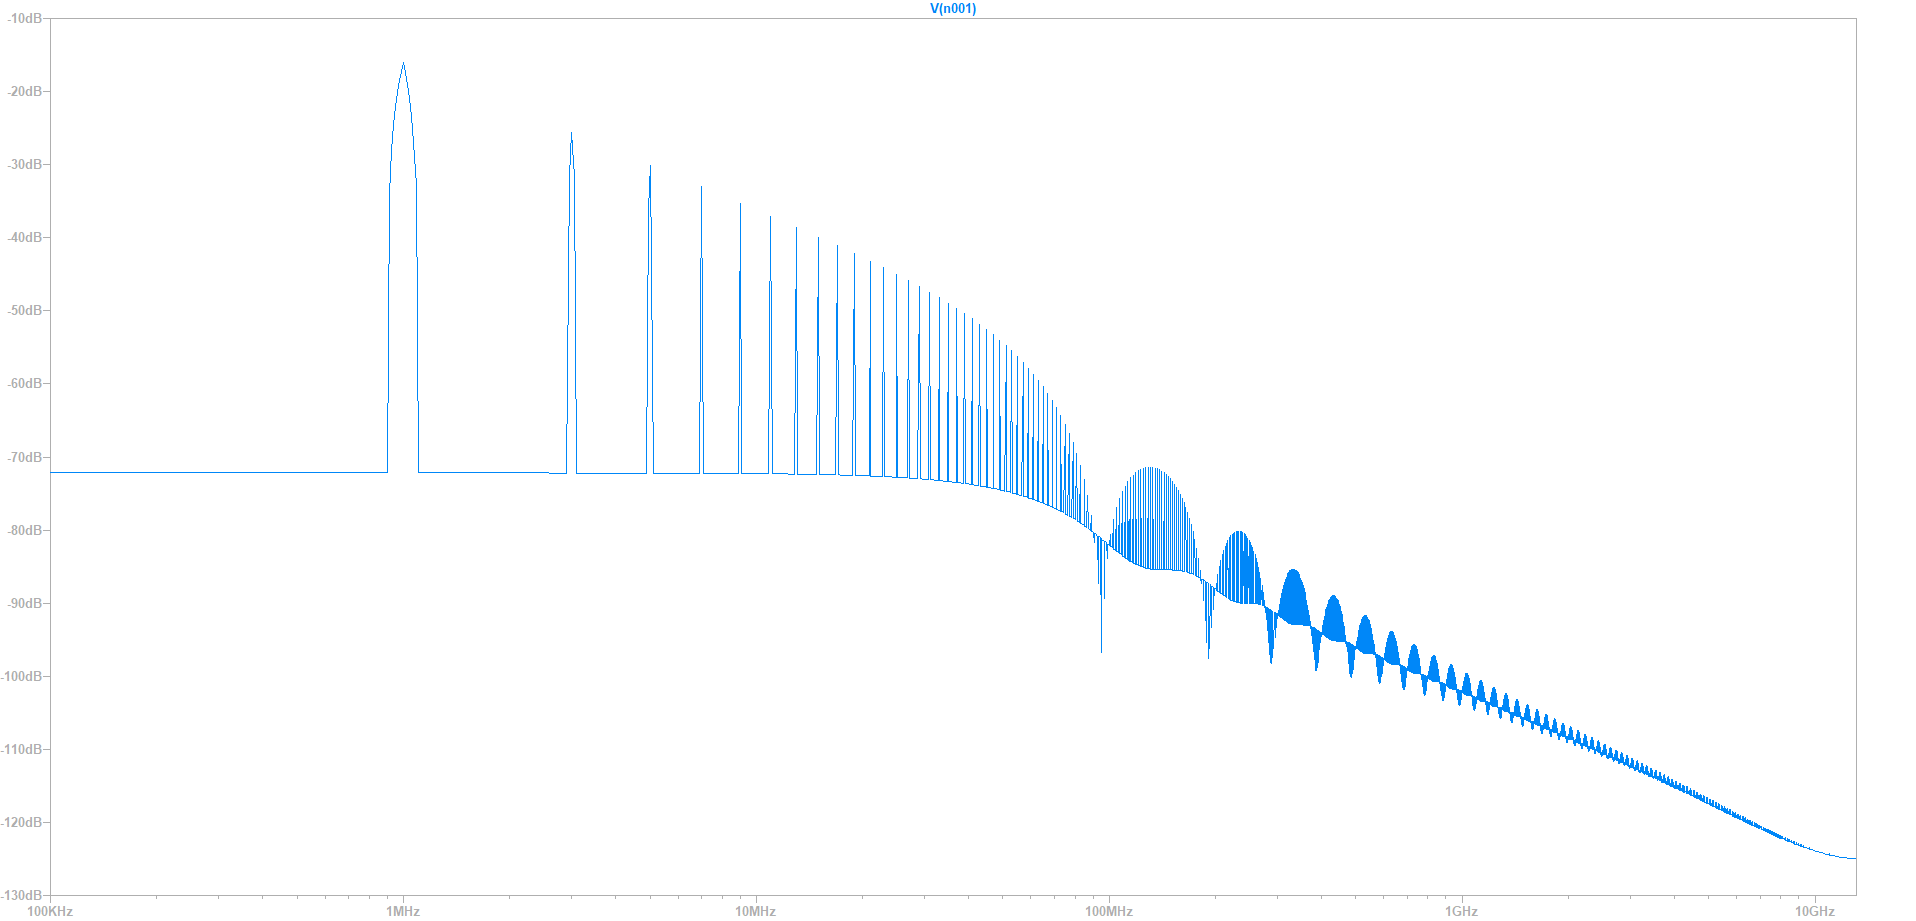
\includegraphics[width=0.9\textwidth]{/ImagenesEjercicio2/FFT-Cuadrada.png}
\caption{Simulación del espectro de una señal cuadrada.}
	\label{fig:simcuad}
\end{figure}


\subsubsection{Medición}
Las mediciones se llevaron a cabo utilizando el marcador del dispositivo el cual al posicionarlo sobre el armónico que se quiere medir muestra la frecuencia y la potencia de este en $dBm$. A continuación se presentan las mediciones realizadas con el analizador de espectro:

\begin{table}[H]
\scalebox{0.8}{
\begin{tabular}{@{}ccccccccccc@{}}
\toprule
$0,982 MHz$ & $1,981 MHz$ & $2,98 MHz$ & $3,98 MHz$ & $4,98MHz$ & $5,979 MHz$ & $6,979 MHz$ & $7,978 MHz$ & $8,979 MHz$ & $9,979 MHz$ & $10,978 MHz$ \\ \midrule
$-11.2dBm$ & $-63dBm$ & $-18.2dBm$ & $-62.8dBm$ & $-22.6dBm$ & $-63.8dBm$ & $-30.2dBm$ & $-63.4dBm$ & $-27.6dBm$ & $-61.4dBm$ & $-32.6dBm$
\end{tabular}
}
\end{table}

Puede observarse cómo los armónicos múltiplos pares de la frecuencia fundamental tienen una potencia muy baja comparado con los impares. Esto se corresponde con la teoría.

\subsubsection{Cálculo del Duty-Cycle}	

Se entiende por duty cycle o ciclo de trabajo a la relación entre el tiempo en que la señal está activa y el período de dicha señal. Expresado en porcentaje, puede variar desde $0\%$ hasta $100\%$. Matemáticamente, para una señal cuadrada el ciclo de trabajo $D$ puede expresarse como $D=\frac{\tau}{T}.100\%$, donde $\tau$ es el tiempo en que la señal está activa y $T$ es el período.

Luego, podemos escribir el pulso cuadrado con un Duty Cycle determinado por $\tau$ como 

\begin{equation}
    x(t)=A\Pi(t-\frac{\tau}{T})
\end{equation}

cuya serie de Fourier puede expresarse como 

\begin{equation}
x(t)=\sum_{n impar}\frac{2A}{\pi n} sin(\frac{\pi n\tau}{T})
\end{equation}

Luego, como los armónicos pares se anulan, tenemos $sin(\frac{\pi n\tau}{T})=0$ si $n=2k$ con $k$ entero. De ahí se deduce que $\frac{\tau}{T}=\frac{1}{2}$, de donde el Duty Cycle es del $50\%$

\subsection{Señal Triangular}

Para esta sección se generó una señal triangular con DC del 50\% utilizando el generador GW.

\subsubsection{Cálculo Analítico}

Para una señal triangular $x(t)$ con amplitud $A$ y frecuencia $f_0$, se tiene que los coeficientes de la serie de Fourier son:

\begin{equation}
    |X_n|=
    \begin{cases}
                  \frac{4A}{\pi^2 n^2}, \text{si n es impar}\\ 
                  0, \text{si n es par} \\
     \end{cases}
\end{equation}

Se observa nuevamente que los armónicos pares valen cero. 

\subsubsection{Simulación del Espectro}

Se simuló el espectro de una señal triangular. Dicho espectro puede observarse en la figura (\ref{fig:simtriang})

\begin{figure}[H]
	\centering
	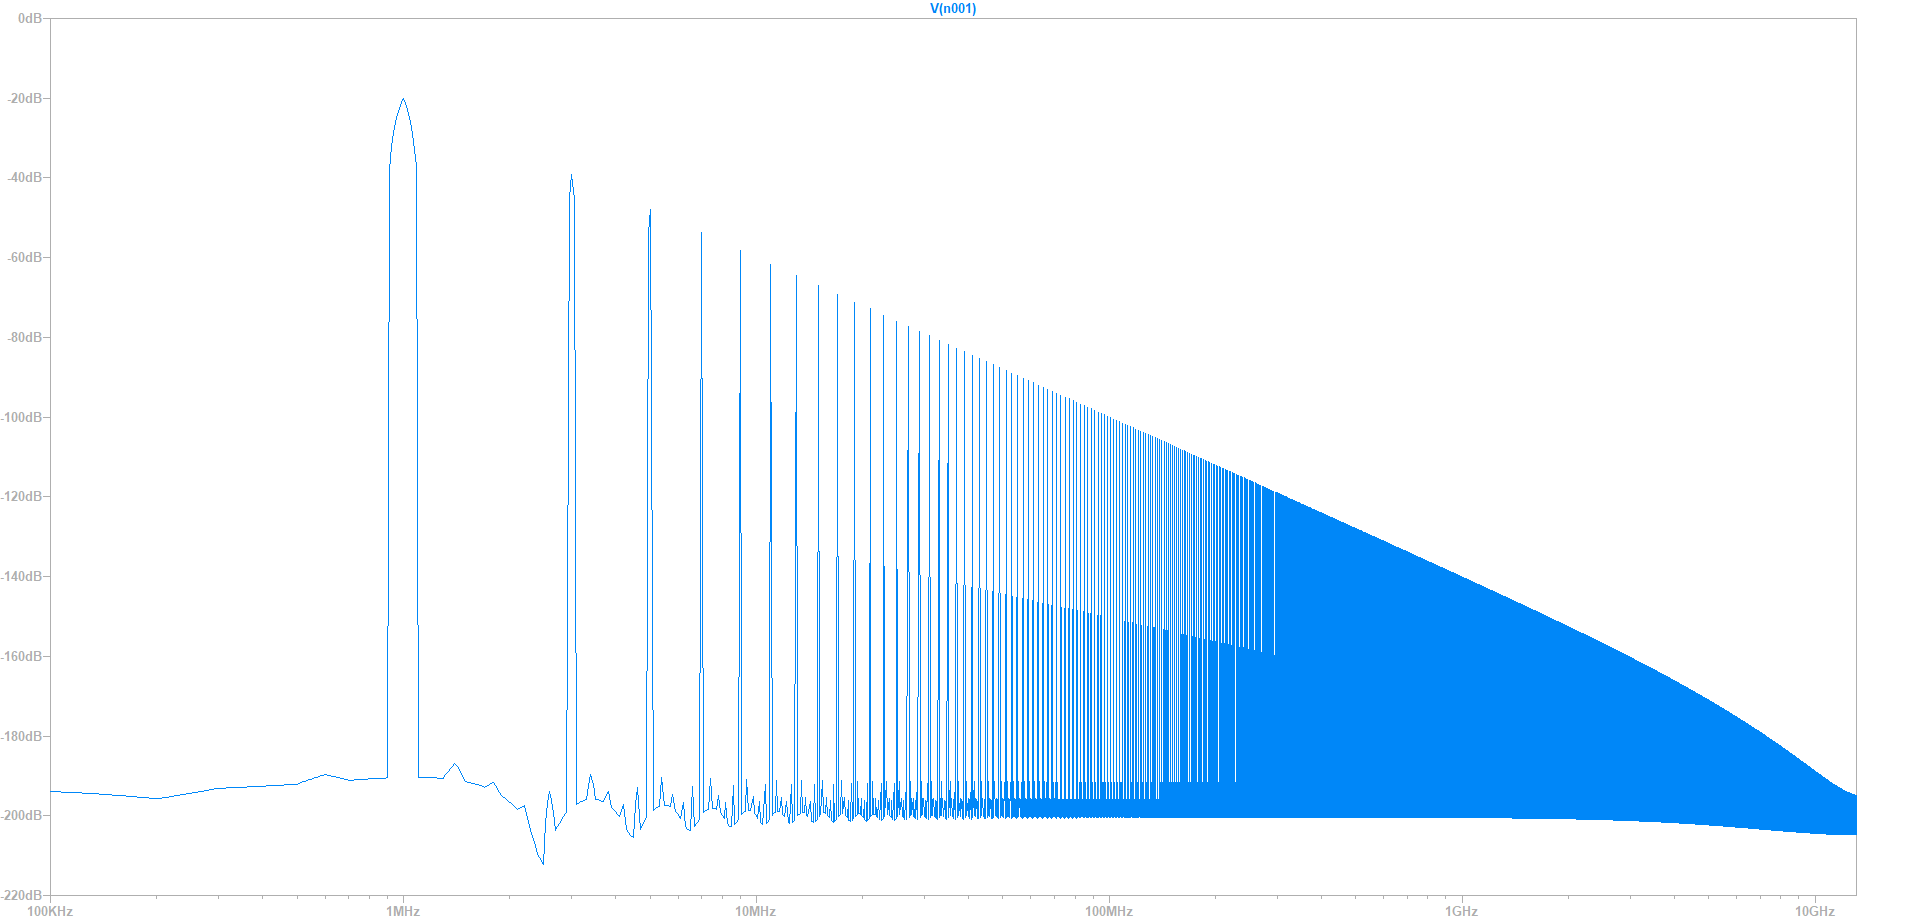
\includegraphics[width=0.9\textwidth]{/ImagenesEjercicio2/FFT-Triangular.png}
\caption{Simulación del espectro de una señal triangular.}
	\label{fig:simtriang}
\end{figure}


\subsubsection{Medición}

De forma similar al caso anterior, se midieron algunos armónicos junto con sus potencias correspondientes (en $dBm$) A continuación se presenta una tabla con las mediciones.



\begin{table}[H]
\scalebox{0.8}{
\begin{tabular}{@{}ccccccccccc@{}}
\toprule
$1,028 MHz$ & $2,027 MHz$ & $3,014 MHz$ & $4,012 MHz$ & $5,026 MHz$ & $6,004 MHz$ & $7,037 MHz$ & $8,007 MHz$ & $9,047 MHz$ & $10,029 MHz$ \\ \midrule

$-13,6dBm$ & $-55dBm$ & $-34dBm$ & $-70dBm$ & $-44,2dBm$ & $-89,6dBm$ & $-53dBm$ & $-$ & $-53,2dBm$ & $-$

\end{tabular}
}
\end{table}

Notemos cómo nuevamente los armónicos pares tienen potencia mucho más baja que los impares. De hecho, los correspondientes a frecuencias de $8,007 MHz$ y $10,029MHz$ no pudieron medirse por ser demasiado tenues.

\subsection{Tren de Pulsos}

Se generó un tren de pulsos con un DC del $33,3\%$. 

\subsubsection{Cálculo Analítico}

De forma análoga a lo desarrollado en la sección de la onda cuadrada, como el DC es del 33,3\% se verifica que $sin(\frac{n\pi}{3}=0$), de donde los armónicos múltiplos de $3$ se anularán. 

Haciendo el desarrollo en serie de Fourier se encuentra que $|X_n|=\frac{A\sqrt{3}}{n\pi}$ para todo $n$ que no sea múltiplo de $3$

\subsubsection{Simulación del Espectro}

Se simuló el espectro del tren de pulsos. El resultado puede observarse en la figura (\ref{fig:simpulso})

\begin{figure}[H]
	\centering
	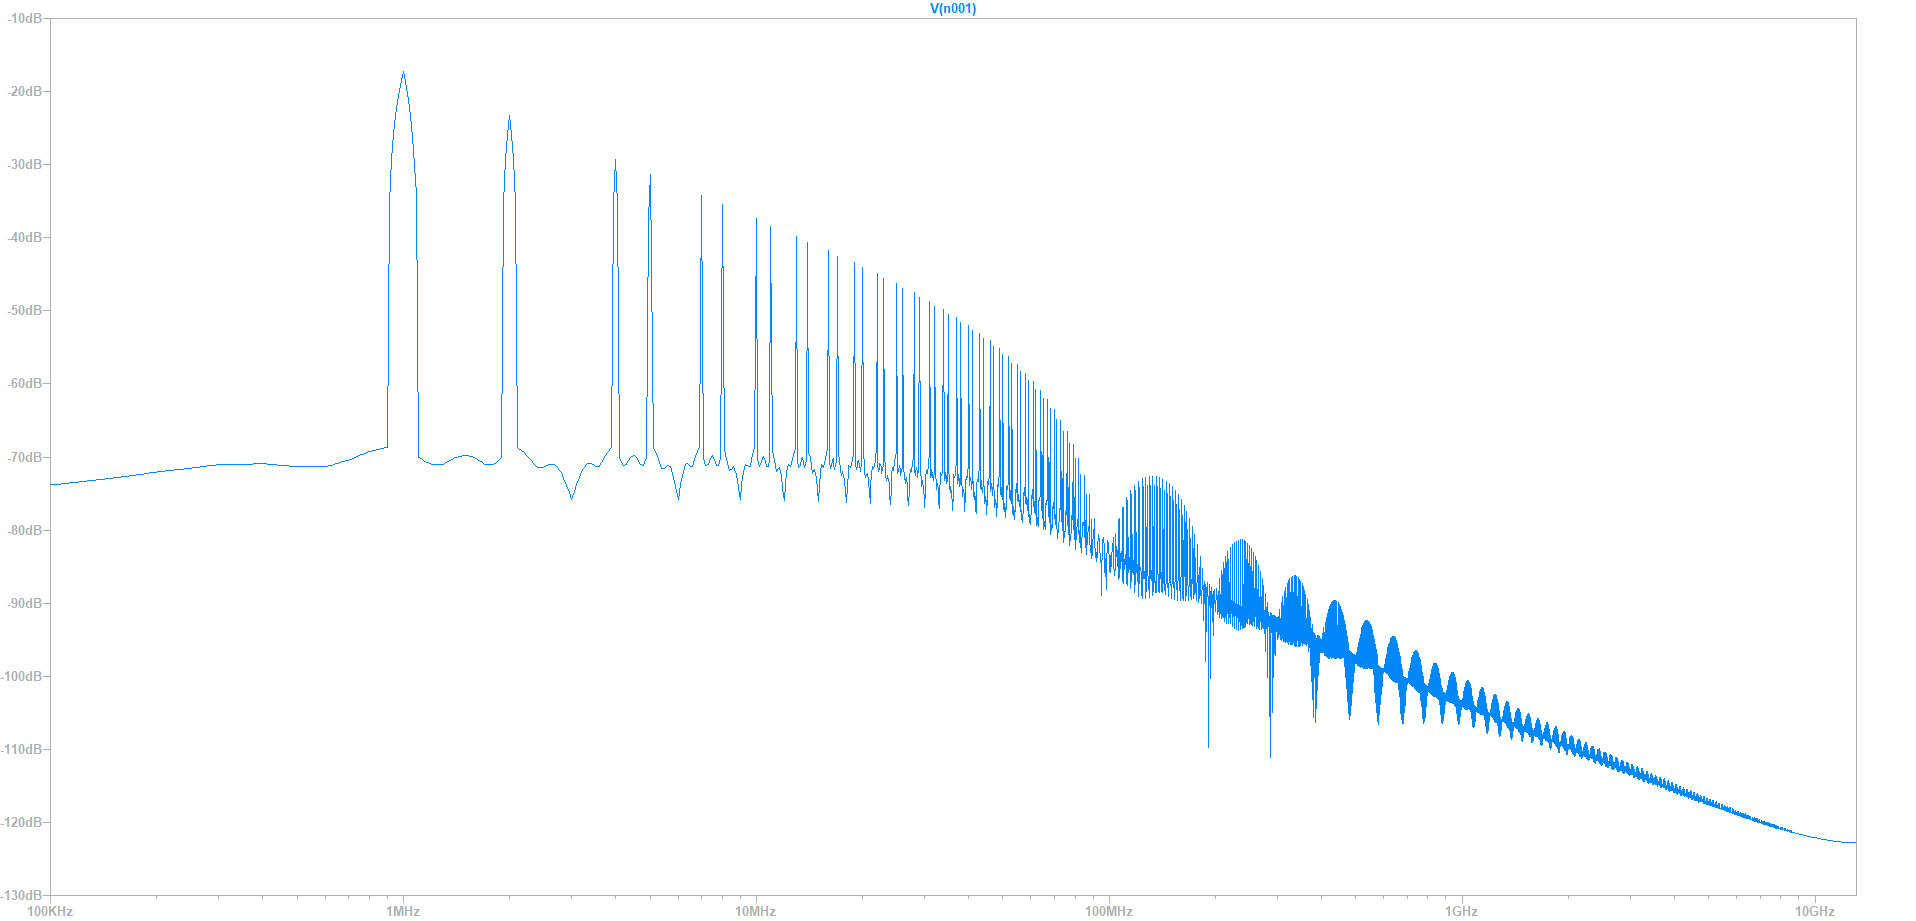
\includegraphics[width=0.9\textwidth]{/ImagenesEjercicio2/FFT-Pulsos.png}
\caption{Simulación del espectro del tren de pulsos}
	\label{fig:simpulso}
\end{figure}

\subsubsection{Medición}

Se midieron los primeros armónicos con sus correspondientes potencias. Se presentan los resultados en la siguiente tabla:

\begin{table}[H]
\scalebox{0.8}{
\begin{tabular}{@{}ccccccccccc@{}}
\toprule
$1,018 MHz$ & $2,018 MHz$ & $3,015 MHz$ & $4,011 MHz$ & $5,009 MHz$ & $6,004 MHz$ & $7,009 MHz$ & $8,007 MHz$ & $9,002 MHz$ & $9,999 MHz$ & $10,998 MHz$ \\ \midrule
$-10,2dBm$ & $-16,2dBm$ & $-63dBm$ & $-25,4dBm$ & $-26,1dBm$ & $-81dBm$ & $-32,2dBm$ & $-34,4dBm$ & $-84,8dBm$ & $-36,8dBm$ & $-31,6dBm$
\end{tabular}
}
\end{table}

Las mediciones corresponden con la teoría. Se puede observar cómo en los armónicos múltiplos de $3$ la potencia cae considerablemente.

\subsection{Conclusiones}

En los tres casos se puede observar que hubo correspondencia entre la teoría y la práctica. Tanto en la cuadrada con DC del $50\%$ como en la triangular la potencia en los armónicos pares decayó considerablemente. Por supuesto, no fue exactamente cero porque el generador es incapaz de crear una onda cuadrada o triangular perfecta; de hecho en el primer ejercicio se vio que tanto el generador Agilent como el GW poseen en mayor o menor medida un grado de distorsión armónica. Una conclusión similar se puede confeccionar para el tren de pulsos: los armónicos múltiplos de tres resultaron tener una potencia que, aunque no fue cero, resultó muy baja comparada con el resto de los armónicos. El analizador de espectros resulta un elemento muy útil a la hora de analizar espectros de señales. No obstante, pueden surgir complicaciones si se intentan medir potencias muy pequeñas, ya que éstas se pueden confundir con el piso de ruido.
